\begin{frame}
    \frametitle{Definición del Problema de SLAM}
    \note{Información extraída de https://www.youtube.com/watch?v=X30sEgIws0g}
    \note{Información extraída de https://www.ipb.uni-bonn.de/html/teaching/photo12-2021/2021-pho2-16-ekf-slam.pptx.pdf}

    Dado:
    \begin{itemize}
        \item Comandos de control enviados
        
        \begin{equation*}
            \controlCommand_{1:T} = \{\controlCommand_1, \controlCommand_2, \ldots, \controlCommand_T\}
        \end{equation*}
        \item Observaciones
        \begin{equation*}
            \observation_{1:T} = \{\observation_1, \observation_2, \ldots, \observation_T\}
        \end{equation*}
    \end{itemize}

    Se busca:
    \begin{itemize}
        \item Mapa del entorno: $\map$
        \item Trayectoria (o pose actual) del vehículo:
        \begin{equation*}
            \state_{0:T} = \{\state_0, \state_1, \ldots, \state_T\} \qquad \text{or} \qquad \state_{t}
        \end{equation*}
    \end{itemize}
\end{frame}

\begin{frame}
    \frametitle{Bayes Filter}
    \note{Información extraída de https://www.youtube.com/watch?v=X30sEgIws0g}
    \note{Información extraída de https://www.ipb.uni-bonn.de/html/teaching/photo12-2021/2021-pho2-16-ekf-slam.pptx.pdf}

    \begin{itemize}
        \item Recursive filter with \textbf{prediction} and \textbf{correction} steps
        \item Estimates: $p(x_t, \map | \observation_{1:t}, \controlCommand_{1:t})$
        \item Kalman Filter is a recursive Bayes Filter for the \textbf{linear Gaussian case}
        \item \textbf{EKF} for dealing with \textbf{non-linearities}
    \end{itemize}
\end{frame}

\begin{frame}
    \frametitle{Grafical Model of Full SLAM}
    \note{Información extraída de https://www.youtube.com/watch?v=X30sEgIws0g}
    \note{Información extraída de https://www.ipb.uni-bonn.de/html/teaching/photo12-2021/2021-pho2-16-ekf-slam.pptx.pdf}

    \[ p(\state_{1:t}, \map | \observation_{1:t}, \controlCommand_{1:t}) \]

    \begin{center}
        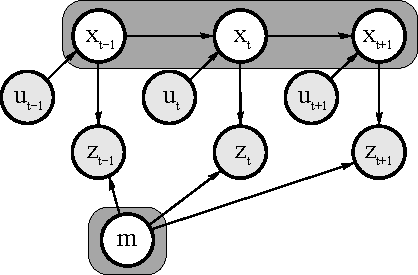
\includegraphics[width=0.6\textwidth]{../images/ekf_slam/graphical_model_full_slam.pdf}
    \end{center}
\end{frame}

\begin{frame}
    \frametitle{Grafical Model of Online SLAM}
    \note{Información extraída de https://www.youtube.com/watch?v=X30sEgIws0g}
    \note{Información extraída de https://www.ipb.uni-bonn.de/html/teaching/photo12-2021/2021-pho2-16-ekf-slam.pptx.pdf}

    We consider the Kalman filter as a solution to the online SLAM problem:
    \begin{equation*}
        p(\state_{t}, \map | \observation_{1:t}, \controlCommand_{1:t}) = \int \int \cdots \int p(\state_{1:t}, \map | \observation_{1:t}, \controlCommand_{1:t}) d\state_{1} d\state_{2} \ldots d\state_{t-1}
    \end{equation*}

    \begin{center}
        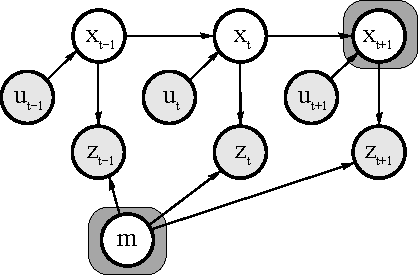
\includegraphics[width=0.6\textwidth]{../images/ekf_slam/graphical_model_online_slam.pdf}
    \end{center}

    \note{EKF can not adjust previous poses of the trajectory when a loop closure is done but can adjust the map and the current pose.}

\end{frame}

\begin{frame}
    \frametitle{Algoritmo de Filtro de Kalman Extendido}
    \note{Información extraída de https://www.youtube.com/watch?v=X30sEgIws0g}
    \note{Información extraída de https://www.ipb.uni-bonn.de/html/teaching/photo12-2021/2021-pho2-16-ekf-slam.pptx.pdf}
    
    \begin{algorithmic}[1]
    \Procedure{ExtendedKalmanFilter}{$\mu_{t-1}, \covariance_{t-1}, \controlCommand_{t}, \observation_{t}$}
        \State $\overline{\mu}_{t} = \motionModelFunction{\controlCommand_{t}, \mu_{t-1}}$
        \State $\overline{\covariance}_{t} = \motionModelJacobian_{t} \covariance_{t-1} \motionModelJacobian_{t}^{\top}+\motionParametersCovariance_{t}$
        \Statex
        \State $\kalmanGain_{t} = \overline{\covariance}_{t} \observationModelJacobian_{t}^{\top} (\observationModelJacobian_{t} \overline{\covariance}_{t}  \observationModelJacobian_{t} + \observationModelCovariance_{t})^{-1} $
        \State $\mu_{t} = \overline{\mu}_{t} + \kalmanGain_{t} (\observation_{t} - \observationModelFunction{\overline{\mu}_{t}})$
        \State $\covariance_{t} =  (I - \kalmanGain_{t} \observationModelJacobian_{t}) \overline{\covariance}_{t}$
        \State \Return $\mu_{t}, \covariance_{t}$
    \EndProcedure
    \end{algorithmic}
\end{frame}

\begin{frame}
    \frametitle{EKF SLAM}
    \note{Información extraída de https://www.youtube.com/watch?v=X30sEgIws0g}
    \note{Información extraída de https://www.ipb.uni-bonn.de/html/teaching/photo12-2021/2021-pho2-16-ekf-slam.pptx.pdf}

    \begin{itemize}
        \item Application of EKF to SLAM
        \item Estimate robot's pose and landmark locations
        \item Assumption: known data association
        \item State space (for the 2D plane) is:
    \end{itemize}
    \[ x_t = (\underbrace{x, y, \theta}_{robot's pose}, \underbrace{\map_{1,x}, \map_{1,y}}_{\text{landmark 1}}, \ldots, \underbrace{\map_{n,x}, \map_{n,y}}_{\text{landmark n}} )^{\top} \]
\end{frame}

\begin{frame}
    \frametitle{EKF SLAM: State Representation}
    \note{Información extraída de https://www.youtube.com/watch?v=X30sEgIws0g}
    \note{Información extraída de https://www.ipb.uni-bonn.de/html/teaching/photo12-2021/2021-pho2-16-ekf-slam.pptx.pdf}

    \begin{itemize}
        \item Map with $n$ landmarks: $(3+2n)$-dimensional Gaussian
        \item Belief represented by:
        \begin{equation*}
            \underbrace{\begin{bNiceMatrix}[margin = 4pt]
                \CodeBefore
                \rectanglecolor{yellow!40}{1-1}{3-1}
                \rectanglecolor{blue!20}{4-1}{9-1}
                \Body
                x \\
                y \\
                \theta \\
                \map_{1,x} \\
                \map_{1,y} \\
                \vdots \\
                \map_{n,x} \\
                \map_{n,y}
            \end{bNiceMatrix}}_{\mu}
            \underbrace{\begin{bNiceMatrix}[margin = 4pt]
                \CodeBefore
                \rectanglecolor{yellow!40}{1-1}{3-3}
                \rectanglecolor{green!40}{1-4}{3-8}
                \rectanglecolor{green!40}{4-1}{8-3}
                \rectanglecolor{blue!20}{4-4}{8-8}
                \Body
                \sigma_{xx} & \sigma_{xy} & \sigma_{x\theta} & \sigma_{x \map_{1,x}} & \sigma_{x \map_{1,y}} & \cdots & \sigma_{x \map_{n,x}} & \sigma_{x \map_{n,y}}\\
                \sigma_{yx} & \sigma_{yy} & \sigma_{y\theta} & \sigma_{y \map_{1,x}} & \sigma_{y \map_{1,y}} & \cdots & \sigma_{y \map_{n,x}} & \sigma_{y \map_{n,y}}\\
                \sigma_{\theta x} & \sigma_{\theta y} & \sigma_{\theta\theta} & \sigma_{\theta \map_{1,x}} & \sigma_{\theta \map_{1,y}} & \cdots & \sigma_{\theta \map_{n,x}} & \sigma_{\theta \map_{n,y}}\\
                \sigma_{\map_{1,x}x} & \sigma_{\map_{1,x}y} & \sigma_{\map_{1,x}\theta} & \sigma_{\map_{1,x}\map_{1,x}} & \sigma_{\map_{1,x}\map_{1,y}} & \cdots & \sigma_{\map_{1,x} \map_{n,x}} & \sigma_{\map_{1,x} \map_{n,y}} \\
                \sigma_{\map_{1,y}x} & \sigma_{\map_{1,y}y} & \sigma_{\map_{1,y}\theta} & \sigma_{\map_{1,y}\map_{1,x}} & \sigma_{\map_{1,y}\map_{1,y}} & \cdots & \sigma_{\map_{1,y} \map_{n,x}} & \sigma_{\map_{1,y} \map_{n,y}} \\
                \vdots & \vdots & \vdots & \vdots & \vdots & \ddots & \vdots & \vdots \\
                \sigma_{\map_{n,x}x} & \sigma_{\map_{n,x}y} & \sigma_{\map_{n,x}\theta} & \sigma_{\map_{n,x} \map_{1,x}} & \sigma_{\map_{n,x} \map_{1,y}} &\cdots & \sigma_{\map_{n,x} \map_{n,x}} & \sigma_{\map_{n,x} \map_{n,y}} \\
                \sigma_{\map_{n,y}x} & \sigma_{\map_{n,y}y} & \sigma_{\map_{n,y}\theta} & \sigma_{\map_{n,y} \map_{1,x}} & \sigma_{\map_{n,y} \map_{1,y}} & \cdots & \sigma_{\map_{n,y} \map_{n,x}} & \sigma_{\map_{n,y} \map_{n,y}}
            \end{bNiceMatrix}}_{\Sigma}
        \end{equation*}
    \end{itemize}
\end{frame}

\begin{frame}
    \frametitle{EKF SLAM: State Representation}
    \note{Información extraída de https://www.youtube.com/watch?v=X30sEgIws0g}
    \note{Información extraída de https://www.ipb.uni-bonn.de/html/teaching/photo12-2021/2021-pho2-16-ekf-slam.pptx.pdf}

    \begin{itemize}
        \item Map with $n$ landmarks: $(3+2n)$-dimensional Gaussian
        \item Belief represented by:
        \begin{equation*}
            \underbrace{\begin{bNiceMatrix}[margin = 4pt]
                \CodeBefore
                \rectanglecolor{yellow!40}{1-1}{1-1}
                \rectanglecolor{blue!20}{2-1}{4-1}
                \Body
                \state_t \\
                \map_1 \\
                \vdots \\
                \map_n
            \end{bNiceMatrix}}_{\mu}
            \underbrace{\begin{bNiceMatrix}[margin = 4pt]
                \CodeBefore
                \rectanglecolor{yellow!40}{1-1}{1-1}
                \rectanglecolor{green!40}{2-1}{4-1}
                \rectanglecolor{green!40}{1-2}{1-4}
                \rectanglecolor{blue!20}{2-2}{4-4}
                \Body
                \Sigma_{\state_t \state_t} & \Sigma_{\state_t \map_1} & \cdots & \Sigma_{\state_t \map_n} \\
                \Sigma_{\map_1 \state_t} & \Sigma_{\map_1 \map_1} & \cdots & \Sigma_{\map_1 \map_n} \\
                \vdots & \vdots & \ddots & \vdots \\
                \Sigma_{\map_n \state_t} & \Sigma_{\map_n \map_1} & \cdots & \Sigma_{\map_n \map_n}
            \end{bNiceMatrix}}_{\Sigma}
        \end{equation*}
    \end{itemize}

    The matrix diagonal blocks (yellow and blue) are the covariance of the pose and landmarks. The green blocks links the landmarks with the pose.

\end{frame}

\begin{frame}
    \frametitle{EKF SLAM: State Representation}
    \note{Información extraída de https://www.youtube.com/watch?v=X30sEgIws0g}
    \note{Información extraída de https://www.ipb.uni-bonn.de/html/teaching/photo12-2021/2021-pho2-16-ekf-slam.pptx.pdf}

    \begin{itemize}
        \item More Compactly
        \begin{equation*}
            \underbrace{\begin{bNiceMatrix}[margin = 4pt]
                \CodeBefore
                \rectanglecolor{yellow!40}{1-1}{1-1}
                \rectanglecolor{blue!20}{2-1}{2-1}
                \Body
                \state\\
                \map
            \end{bNiceMatrix}}_{\mu}
            \underbrace{\begin{bNiceMatrix}[margin = 4pt]
                \CodeBefore
                \rectanglecolor{yellow!40}{1-1}{1-1}
                \rectanglecolor{green!40}{2-1}{2-1}
                \rectanglecolor{green!40}{1-2}{1-2}
                \rectanglecolor{blue!20}{2-2}{2-2}
                \Body
                \Sigma_{\state \state} & \Sigma_{\state \map} \\
                \Sigma_{\map \state} & \Sigma_{\map \map}
            \end{bNiceMatrix}}_{\Sigma}
        \end{equation*}
    \end{itemize}
\end{frame}

\begin{frame}
    \frametitle{EKF SLAM: Filter Cycle}
    \note{Información extraída de https://www.youtube.com/watch?v=X30sEgIws0g}
    \note{Información extraída de https://www.ipb.uni-bonn.de/html/teaching/photo12-2021/2021-pho2-16-ekf-slam.pptx.pdf}
    \begin{enumerate}
    \item State prediction
    \item Measurement prediction
    \item Measurement
    \item Data association
    \item Update
    \end{enumerate}
\end{frame}

\begin{frame}
    \frametitle{EKF SLAM: Initial State}
    \note{Información extraída de https://www.youtube.com/watch?v=X30sEgIws0g}
    \note{Información extraída de https://www.ipb.uni-bonn.de/html/teaching/photo12-2021/2021-pho2-16-ekf-slam.pptx.pdf}


    \begin{center}
        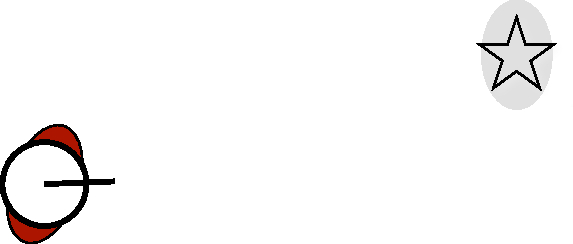
\includegraphics[width=0.4\textwidth]{./ekf_slam/ekf_slam_initial_state.pdf}
    \end{center}

    \begin{equation*}
        \underbrace{\begin{bNiceMatrix}
            \state_t \\
            \map_1 \\
            \vdots \\
            \map_n
        \end{bNiceMatrix}}_{\mu}
        \underbrace{\begin{bNiceMatrix}
            \Sigma_{\state_t \state_t} & \Sigma_{\state_t \map_1} & \cdots & \Sigma_{\state_t \map_n} \\
            \Sigma_{\map_1 \state_t} & \Sigma_{\map_1 \map_1} & \cdots & \Sigma_{\map_1 \map_n} \\
            \vdots & \vdots & \ddots & \vdots \\
            \Sigma_{\map_n \state_t} & \Sigma_{\map_n \map_1} & \cdots & \Sigma_{\map_n \map_n}
        \end{bNiceMatrix}}_{\Sigma}
    \end{equation*}
\end{frame}

\begin{frame}
    \frametitle{EKF SLAM: Predicted Motion}
    \note{Información extraída de https://www.youtube.com/watch?v=X30sEgIws0g}
    \note{Información extraída de https://www.ipb.uni-bonn.de/html/teaching/photo12-2021/2021-pho2-16-ekf-slam.pptx.pdf}


    \begin{center}
        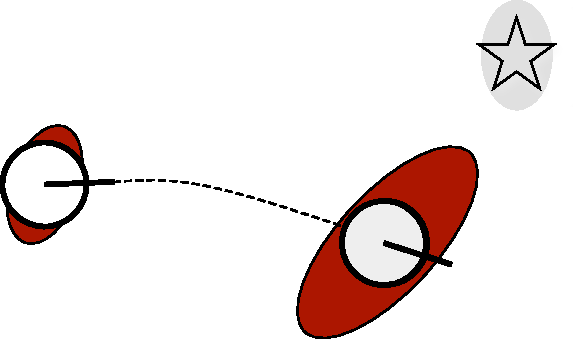
\includegraphics[width=0.4\textwidth]{../images/ekf_slam/ekf_slam_predicted_motion.pdf}
    \end{center}

    \begin{equation*}
        \underbrace{\begin{bNiceMatrix}[margin = 4pt]
            \CodeBefore
            \rectanglecolor{green!40}{1-1}{1-1}
            \Body
            \state_t \\
            \map_1 \\
            \vdots \\
            \map_n
        \end{bNiceMatrix}}_{\mu}
        \underbrace{\begin{bNiceMatrix}[margin = 4pt]
            \CodeBefore
            \rectanglecolor{green!40}{1-1}{1-4}
            \rectanglecolor{green!40}{1-1}{4-1}
            \Body
            \Sigma_{\state_t \state_t} & \Sigma_{\state_t \map_1} & \cdots & \Sigma_{\state_t \map_n} \\
            \Sigma_{\map_1 \state_t} & \Sigma_{\map_1 \map_1} & \cdots & \Sigma_{\map_1 \map_n} \\
            \vdots & \vdots & \ddots & \vdots \\
            \Sigma_{\map_n \state_t} & \Sigma_{\map_n \map_1} & \cdots & \Sigma_{\map_n \map_n}
        \end{bNiceMatrix}}_{\Sigma}
    \end{equation*}

    \tiny

    If the robot moves, the uncertainty increases and we must update the robot pose and the correlation between the robot and the landmarks. The latter happens because now the pose provides less information about the landmarks since the robot got more uncertainty about its pose. The landmarks are not updated since the robot motion does not affect the position of the landmarks.

\end{frame}

\begin{frame}
    \frametitle{EKF SLAM: Predicted Measurement}
    \note{Información extraída de https://www.youtube.com/watch?v=X30sEgIws0g}
    \note{Información extraída de https://www.ipb.uni-bonn.de/html/teaching/photo12-2021/2021-pho2-16-ekf-slam.pptx.pdf}

    Given the predicted pose and the landmark location, we predict the measurement we should obtain.

    \begin{center}
        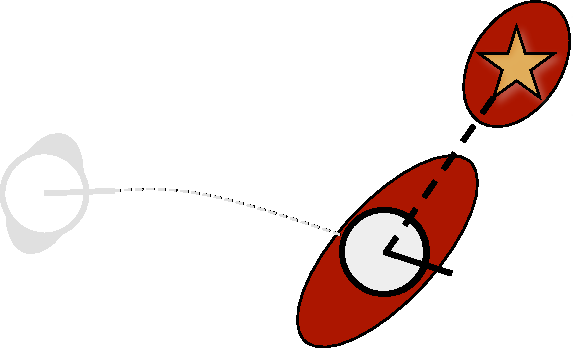
\includegraphics[width=0.4\textwidth]{../images/ekf_slam/ekf_slam_predicted_measurement.pdf}
    \end{center}

    \begin{equation*}
        \underbrace{\begin{bNiceMatrix}
            \state_t \\
            \map_1 \\
            \vdots \\
            \map_n
        \end{bNiceMatrix}}_{\mu}
        \underbrace{\begin{bNiceMatrix}
            \Sigma_{\state_t \state_t} & \Sigma_{\state_t \map_1} & \cdots & \Sigma_{\state_t \map_n} \\
            \Sigma_{\map_1 \state_t} & \Sigma_{\map_1 \map_1} & \cdots & \Sigma_{\map_1 \map_n} \\
            \vdots & \vdots & \ddots & \vdots \\
            \Sigma_{\map_n \state_t} & \Sigma_{\map_n \map_1} & \cdots & \Sigma_{\map_n \map_n}
        \end{bNiceMatrix}}_{\Sigma}
    \end{equation*}
\end{frame}

\begin{frame}
    \frametitle{EKF SLAM: Obtained Measurement}
    \note{Información extraída de https://www.youtube.com/watch?v=X30sEgIws0g}
    \note{Información extraída de https://www.ipb.uni-bonn.de/html/teaching/photo12-2021/2021-pho2-16-ekf-slam.pptx.pdf}

    The sensor observes the landmark.

    \begin{center}
        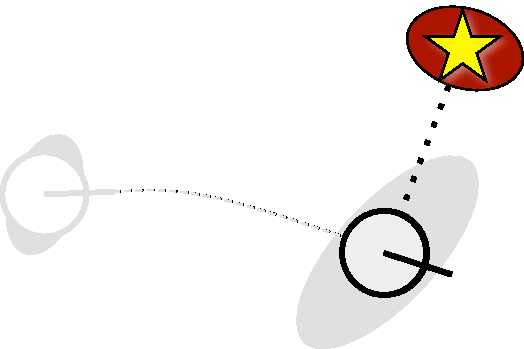
\includegraphics[width=0.4\textwidth]{../images/ekf_slam/ekf_slam_obtained_measurement.pdf}
    \end{center}

    \begin{equation*}
        \underbrace{\begin{bNiceMatrix}
            \state_t \\
            \map_1 \\
            \vdots \\
            \map_n
        \end{bNiceMatrix}}_{\mu}
        \underbrace{\begin{bNiceMatrix}
            \Sigma_{\state_t \state_t} & \Sigma_{\state_t \map_1} & \cdots & \Sigma_{\state_t \map_n} \\
            \Sigma_{\map_1 \state_t} & \Sigma_{\map_1 \map_1} & \cdots & \Sigma_{\map_1 \map_n} \\
            \vdots & \vdots & \ddots & \vdots \\
            \Sigma_{\map_n \state_t} & \Sigma_{\map_n \map_1} & \cdots & \Sigma_{\map_n \map_n}
        \end{bNiceMatrix}}_{\Sigma}
    \end{equation*}
\end{frame}

\begin{frame}
    \frametitle{EKF SLAM: Data Association and Difference Between $h(x)$ and $\observation$}
    \note{Información extraída de https://www.youtube.com/watch?v=X30sEgIws0g}
    \note{Información extraída de https://www.ipb.uni-bonn.de/html/teaching/photo12-2021/2021-pho2-16-ekf-slam.pptx.pdf}

    \begin{center}
        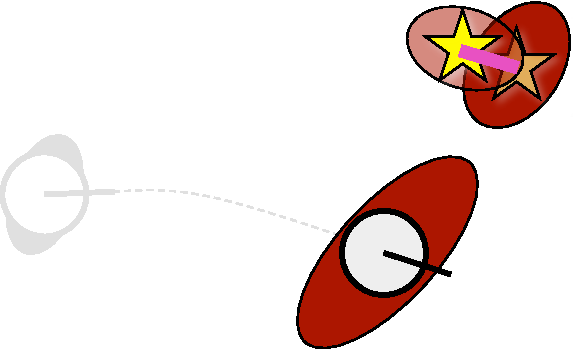
\includegraphics[width=0.4\textwidth]{../images/ekf_slam/ekf_slam_difference_between_prediction_observation.pdf}
    \end{center}

    \begin{equation*}
        \underbrace{\begin{bNiceMatrix}
            \state_t \\
            \map_1 \\
            \vdots \\
            \map_n
        \end{bNiceMatrix}}_{\mu}
        \underbrace{\begin{bNiceMatrix}
            \Sigma_{\state_t \state_t} & \Sigma_{\state_t \map_1} & \cdots & \Sigma_{\state_t \map_n} \\
            \Sigma_{\map_1 \state_t} & \Sigma_{\map_1 \map_1} & \cdots & \Sigma_{\map_1 \map_n} \\
            \vdots & \vdots & \ddots & \vdots \\
            \Sigma_{\map_n \state_t} & \Sigma_{\map_n \map_1} & \cdots & \Sigma_{\map_n \map_n}
        \end{bNiceMatrix}}_{\Sigma}
    \end{equation*}
\end{frame}

\begin{frame}
    \frametitle{EKF SLAM: Update Step}
    \note{Información extraída de https://www.youtube.com/watch?v=X30sEgIws0g}
    \note{Información extraída de https://www.ipb.uni-bonn.de/html/teaching/photo12-2021/2021-pho2-16-ekf-slam.pptx.pdf}


    \begin{center}
        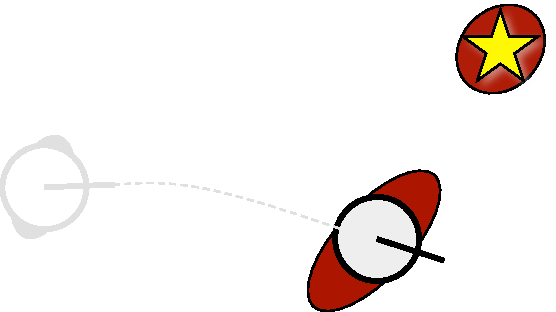
\includegraphics[width=0.4\textwidth]{../images/ekf_slam/ekf_slam_update.pdf}
    \end{center}

    \begin{equation*}
        \underbrace{\begin{bNiceMatrix}[margin = 4pt]
            \CodeBefore
            \rectanglecolor{green!40}{1-1}{4-1}
            \Body
            \state_t \\
            \map_1 \\
            \vdots \\
            \map_n
        \end{bNiceMatrix}}_{\mu}
        \underbrace{\begin{bNiceMatrix}[margin = 4pt]
            \CodeBefore
            \rectanglecolor{green!40}{1-1}{4-4}
            \Body
            \Sigma_{\state_t \state_t} & \Sigma_{\state_t \map_1} & \cdots & \Sigma_{\state_t \map_n} \\
            \Sigma_{\map_1 \state_t} & \Sigma_{\map_1 \map_1} & \cdots & \Sigma_{\map_1 \map_n} \\
            \vdots & \vdots & \ddots & \vdots \\
            \Sigma_{\map_n \state_t} & \Sigma_{\map_n \map_1} & \cdots & \Sigma_{\map_n \map_n}
        \end{bNiceMatrix}}_{\Sigma}
    \end{equation*}

    The robot pose and the landmarks locations are corrected along the whole covariance matrix.
\end{frame}

\begin{frame}
    \frametitle{EKF SLAM: Concrete Example}
    \note{Información extraída de https://www.youtube.com/watch?v=X30sEgIws0g}
    \note{Información extraída de https://www.ipb.uni-bonn.de/html/teaching/photo12-2021/2021-pho2-16-ekf-slam.pptx.pdf}

    Setup:
    \begin{itemize}
        \item Platform moves in the 2D plane
        \item Velocity-based motion model
        \item Observation of point landmarks (e.g. corners or columns)
        \item Range-bearing sensor (measures distance and angle to landmarks)
        \item Known data association (which measurement comes from which landmark)
        \item Known number of landmarks (This is not a constraint but its implementation need some checks in the algorithm: check if the state vector is full requiring to do some bookkeeping). \note{We leave it out of this lecture because It will drag away the attention to the important concepts.}
    \end{itemize}
\end{frame}

\begin{frame}
    \frametitle{Initialization}
    \note{Información extraída de https://www.youtube.com/watch?v=X30sEgIws0g}
    \note{Información extraída de https://www.ipb.uni-bonn.de/html/teaching/photo12-2021/2021-pho2-16-ekf-slam.pptx.pdf}

    \begin{itemize}
        \item Platform starts in its own reference frame
        \item All landmarks are initially unknown (not yet observed)
        \item State vector dimension: $2N + 3$ \\
        (3 for robot pose + $2N$ for $N$ landmarks in 2D space)
        \begin{equation*}
            \mu_0 =
            \begin{bmatrix}
                0 & 0 & 0 & \dots & 0    
            \end{bmatrix}^{\top}
        \end{equation*}
    \end{itemize}
    
    \begin{equation*}
        \Sigma_0 =
        \begin{bmatrix}
            \Sigma_{x_0} & 0 & \cdots & 0 \\
            0 & \infty I_{2} & \cdots & 0 \\
            \vdots & \vdots & \ddots & \vdots \\
            0 & 0 & \cdots & \infty I_{2}
        \end{bmatrix}
    \end{equation*}
    
    \begin{itemize}
        \item $\Sigma_{x_0}$: Initial uncertainty in robot pose (typically  a zero matrix or small)
        \item $\infty I_{2}$: Infinite uncertainty for unobserved landmarks (In practice we don't use infinite to avoid numerical issues)
    \end{itemize}

    \note{We can limit the use of landmark by their index. Each time the landmark a new landmark is observed we increase the index so that landmark is incorporated to the state and the covariance matrix. We do this until we reach the maximum of landmarks that we can work with.}

\end{frame}

\begin{frame}
    \frametitle{Algoritmo de Filtro de Kalman Extendido}
    \note{Información extraída de https://www.youtube.com/watch?v=X30sEgIws0g}
    \note{Información extraída de https://www.ipb.uni-bonn.de/html/teaching/photo12-2021/2021-pho2-16-ekf-slam.pptx.pdf}
    
    \begin{algorithmic}[1]
    \Procedure{ExtendedKalmanFilter}{$\mu_{t-1}, \covariance_{t-1}, \controlCommand_{t}, \observation_{t}$}
        \State $\overline{\mu}_{t} = \alert{\motionModelFunction{\controlCommand_{t}, \mu_{t-1}}}$
        \State $\overline{\covariance}_{t} = \motionModelJacobian_{t} \covariance_{t-1} \motionModelJacobian_{t}^{\top}+\motionParametersCovariance_{t}$
        \Statex
        \State $\kalmanGain_{t} = \overline{\covariance}_{t} \observationModelJacobian_{t}^{\top} (\observationModelJacobian_{t} \overline{\covariance}_{t}  \observationModelJacobian_{t} + \observationModelCovariance_{t})^{-1} $
        \State $\mu_{t} = \overline{\mu}_{t} + \kalmanGain_{t} (\observation_{t} - \observationModelFunction{\overline{\mu}_{t}})$
        \State $\covariance_{t} =  (I - \kalmanGain_{t} \observationModelJacobian_{t}) \overline{\covariance}_{t}$
        \State \Return $\mu_{t}, \covariance_{t}$
    \EndProcedure
    \end{algorithmic}
\end{frame}

\begin{frame}
    \frametitle{Prediction Step (Motion)}
    \note{Información extraída de https://www.youtube.com/watch?v=X30sEgIws0g}
    \note{Información extraída de https://www.ipb.uni-bonn.de/html/teaching/photo12-2021/2021-pho2-16-ekf-slam.pptx.pdf}

    \begin{itemize}
        \item Goa: Update the state space based on the motion
        \item Motion in the plane (with a differential drive robot):
        \begin{equation*}
            \begin{bmatrix} x' \\ y' \\ \theta' \end{bmatrix} = 
            \underbrace{\begin{bmatrix} x \\ y \\ \theta \end{bmatrix} + 
            \begin{bmatrix} 
            -\frac{v_t}{\omega_t} \sin \theta + \frac{v_t}{\omega_t} \sin (\theta + \omega_t \Delta t) \\ 
            \frac{v_t}{\omega_t} \cos \theta - \frac{v_t}{\omega_t} \cos (\theta + \omega_t \Delta t) \\ 
            \omega_t \Delta t 
            \end{bmatrix}}_{g_{x,y,\theta}\left(\controlCommand_{t}, \begin{bmatrix} x & y & \theta \end{bmatrix}^{\top}\right)}
        \end{equation*}
        \item How to map that to the $2N+3$ dimmension state space used in EKF?
    \end{itemize}

\end{frame}

\begin{frame}
    \frametitle{Update the State Space}
    \note{Información extraída de https://www.youtube.com/watch?v=X30sEgIws0g}
    \note{Información extraída de https://www.ipb.uni-bonn.de/html/teaching/photo12-2021/2021-pho2-16-ekf-slam.pptx.pdf}

    \begin{itemize}
        \item From the motion in the plane
        
        \begin{equation*}
            \begin{bmatrix} x' \\ y' \\ \theta' \end{bmatrix} = 
            \underbrace{\begin{bmatrix} x \\ y \\ \theta \end{bmatrix} + 
            \begin{bmatrix} 
            -\frac{v_t}{\omega_t} \sin \theta + \frac{v_t}{\omega_t} \sin (\theta + \omega_t \Delta t) \\ 
            \frac{v_t}{\omega_t} \cos \theta - \frac{v_t}{\omega_t} \cos (\theta + \omega_t \Delta t) \\ 
            \omega_t \Delta t 
            \end{bmatrix}}_{g_{x,y,\theta}\left(\controlCommand_{t}, \begin{bmatrix} x, y, \theta \end{bmatrix}^{\top}\right)}
        \end{equation*}
    

        \item To the \(2N+3\) dimensional space:
        \begin{equation*}
            \begin{bmatrix}
            x' \\
            y' \\
            \theta'\\
            \vdots
            \end{bmatrix}
            =
            \underbrace{\begin{bmatrix}
            x \\
            y \\
            \theta\\
            \vdots
            \end{bmatrix}
            +
            \underbrace{\begin{bNiceMatrix}[margin = 3 pt]
            1 & 0 & 0 & 0 & \ldots & 0 \\
            0 & 1 & 0 & 0 & \ldots & 0 \\
            0 & 0 & 1 & 0 & \ldots & 0 \\
            & & & & &
            \CodeAfter
            \UnderBrace{3-4}{3-6}{2N cols}
            \end{bNiceMatrix}^{\top}}_{F_{x}^{\top}}
            \begin{bmatrix}
            -\frac{v_t}{\omega_t} \sin \theta + \frac{v_t}{\omega_t} \sin (\theta + \omega_t \Delta t) \\
            \frac{v_t}{\omega_t} \cos \theta - \frac{v_t}{\omega_t} \cos (\theta + \omega_t \Delta t) \\
            \omega_t \Delta t
            \end{bmatrix}}_{g(\controlCommand_{t}, \state_t)}
        \end{equation*}
    \end{itemize}

    \note{F is the mapping function that allows to update the state only in the pose components using the motion model.}
\end{frame}

\begin{frame}
    \frametitle{Algoritmo de Filtro de Kalman Extendido}
    \note{Información extraída de https://www.youtube.com/watch?v=X30sEgIws0g}
    \note{Información extraída de https://www.ipb.uni-bonn.de/html/teaching/photo12-2021/2021-pho2-16-ekf-slam.pptx.pdf}
    
    \begin{algorithmic}[1]
    \Procedure{ExtendedKalmanFilter}{$\mu_{t-1}, \covariance_{t-1}, \controlCommand_{t}, \observation_{t}$}
        \State $\overline{\mu}_{t} = \motionModelFunction{\controlCommand_{t}, \mu_{t-1}}$
        \State $\alert{\overline{\covariance}_{t} = \motionModelJacobian_{t} \covariance_{t-1} \motionModelJacobian_{t}^{\top}+\motionParametersCovariance_{t}}$
        \Statex
        \State $\kalmanGain_{t} = \overline{\covariance}_{t} \observationModelJacobian_{t}^{\top} (\observationModelJacobian_{t} \overline{\covariance}_{t}  \observationModelJacobian_{t} + \observationModelCovariance_{t})^{-1} $
        \State $\mu_{t} = \overline{\mu}_{t} + \kalmanGain_{t} (\observation_{t} - \observationModelFunction{\overline{\mu}_{t}})$
        \State $\covariance_{t} =  (I - \kalmanGain_{t} \observationModelJacobian_{t}) \overline{\covariance}_{t}$
        \State \Return $\mu_{t}, \covariance_{t}$
    \EndProcedure
    \end{algorithmic}
\end{frame}

\begin{frame}
    \frametitle{Update Covariance}
    \note{Información extraída de https://www.youtube.com/watch?v=X30sEgIws0g}
    \note{Información extraída de https://www.ipb.uni-bonn.de/html/teaching/photo12-2021/2021-pho2-16-ekf-slam.pptx.pdf}

    \begin{itemize}
        \item The function $g$ only affects de motion and not the landmarks
    \end{itemize}

    Jacobian:
    \begin{equation*}
        G_t = 
        \begin{bmatrix}
            G_{t}^{\state} & 0 \\
            0 & I
        \end{bmatrix}
    \end{equation*}
    where $G_{t}^{\state}$ is the $3 \times 3$ Jacobian of the motion and $I$ is the $2N \times 2N$ identity matrix.


    Note that the Identity submatrix $I$ means that landmarks covariances would not change (it would remains the same as the previous covariance).

\end{frame}

\begin{frame}
    \frametitle{Jacobian of the Motion}
    \note{Información extraída de https://www.youtube.com/watch?v=X30sEgIws0g}
    \note{Información extraída de https://www.ipb.uni-bonn.de/html/teaching/photo12-2021/2021-pho2-16-ekf-slam.pptx.pdf}
    
    The Jacobian matrix $G_{t}^{\state}$ for the motion model is computed as:
    
    \begin{align*}
        G_{t}^{\state} &= \frac{\partial}{\partial(x, y, \theta)^{\top}} \left(
        \begin{bmatrix}
        x \\
        y \\
        \theta
        \end{bmatrix}
        +
        \begin{bmatrix}
        -\frac{v_t}{\omega_t} \sin \theta + \frac{v_t}{\omega_t} \sin(\theta + \omega_t \Delta t) \\
        \frac{v_t}{\omega_t} \cos \theta - \frac{v_t}{\omega_t} \cos(\theta + \omega_t \Delta t) \\
        \omega_t \Delta t
        \end{bmatrix}
        \right) \\
        &= I + \frac{\partial}{\partial(x, y, \theta)^{\top}} 
        \begin{bmatrix}
        -\frac{v_t}{\omega_t} \sin \theta + \frac{v_t}{\omega_t} \sin(\theta + \omega_t \Delta t) \\
        \frac{v_t}{\omega_t} \cos \theta - \frac{v_t}{\omega_t} \cos(\theta + \omega_t \Delta t) \\
        \omega_t \Delta t
        \end{bmatrix} \\
        &= I + 
        \begin{bmatrix}
        0 & 0 & -\frac{v_t}{\omega_t} \cos \theta + \frac{v_t}{\omega_t} \cos(\theta + \omega_t \Delta t) \\
        0 & 0 & -\frac{v_t}{\omega_t} \sin \theta + \frac{v_t}{\omega_t} \sin(\theta + \omega_t \Delta t) \\
        0 & 0 & 0
        \end{bmatrix} \\
        &= 
        \begin{bmatrix}
        1 & 0 & -\frac{v_t}{\omega_t} \cos \theta + \frac{v_t}{\omega_t} \cos(\theta + \omega_t \Delta t) \\
        0 & 1 & -\frac{v_t}{\omega_t} \sin \theta + \frac{v_t}{\omega_t} \sin(\theta + \omega_t \Delta t) \\
        0 & 0 & 1
        \end{bmatrix}
    \end{align*}
    
\end{frame}

\begin{frame}
    \frametitle{This leads to the Covariance update}
    \note{Información extraída de https://www.youtube.com/watch?v=X30sEgIws0g}
    \note{Información extraída de https://www.ipb.uni-bonn.de/html/teaching/photo12-2021/2021-pho2-16-ekf-slam.pptx.pdf}

    \begin{align*}
        \bar{\Sigma}_t &= G_t \Sigma_{t-1} G_t^{\top} + R_t \\
        &= 
        \begin{bmatrix}
        G_{t}^{\state} & 0 \\
        0 & I
        \end{bmatrix}
        \begin{bmatrix}
        \Sigma_{xx} & \Sigma_{xm} \\
        \Sigma_{mx} & \Sigma_{mm}
        \end{bmatrix}
        \begin{bmatrix}
        (G_{t}^{\state})^{\top} & 0 \\
        0 & I
        \end{bmatrix}
        + R_t \\
        &=
        \begin{bmatrix}
        G_{t}^{\state} \Sigma_{xx} (G_{t}^{\state})^{\top} & G_{t}^{\state} \Sigma_{xm} \\
        (G_{t}^{\state} \Sigma_{xm})^{\top} & \Sigma_{mm}
        \end{bmatrix}
        + R_t
    \end{align*}

\end{frame}

\begin{frame}
    \frametitle{EKF SLAM: Prediction Step}
    \note{Información extraída de https://www.youtube.com/watch?v=X30sEgIws0g}
    \note{Información extraída de https://www.ipb.uni-bonn.de/html/teaching/photo12-2021/2021-pho2-16-ekf-slam.pptx.pdf}

    \begin{algorithmic}[1]
        \Procedure{EKF\_SLAM\_Prediction}{$\mu_{t-1}, \Sigma_{t-1}, \controlCommand_t, \observation_t, c_t, R_t$}
        \State $F_{\state} = \begin{bmatrix}
        1 & 0 & 0 & 0 & 0 & \cdots & 0 \\
        0 & 1 & 0 & 0 & 0 & \cdots & 0 \\
        0 & 0 & 1 & 0 & 0 & \cdots & 0 \\
        \end{bmatrix}$
        \vspace{1em}
        \State $\bar{\mu}_t = \mu_{t-1} + F_x^{\top}
        \begin{bmatrix}
        \frac{-v_t}{\omega_t} \sin(\mu_{t-1,\theta}) + \frac{v_t}{\omega_t} \sin(\mu_{t-1,\theta} + \omega_t \Delta t) \\
        \frac{v_t}{\omega_t} \cos(\mu_{t-1,\theta}) - \frac{v_t}{\omega_t} \cos(\mu_{t-1,\theta} + \omega_t \Delta t) \\
        \omega_t \Delta t
        \end{bmatrix}$
        \vspace{1em}
        \State $G_t = I + F_{\state}^{\top}
        \begin{bmatrix}
        0 & 0 & \frac{-v_t}{\omega_t} \cos(\mu_{t-1,\theta}) + \frac{v_t}{\omega_t} \cos(\mu_{t-1,\theta} + \omega_t \Delta t) \\
        0 & 0 & \frac{-v_t}{\omega_t} \sin(\mu_{t-1,\theta}) + \frac{v_t}{\omega_t} \sin(\mu_{t-1,\theta} + \omega_t \Delta t) \\
        0 & 0 & 0
        \end{bmatrix} F_{\state}$
        \vspace{1em}
        \State $\bar{\Sigma}_t = G_{t} \Sigma_{t-1} G_{t}^{\top} + \underbrace{F_{\state}^{\top} R_{t}^{\state} F_{\state}}_{R_t}$
        \EndProcedure
    \end{algorithmic}
    
\end{frame}

\begin{frame}
    \frametitle{Algoritmo de Filtro de Kalman Extendido}
    \note{Información extraída de https://www.youtube.com/watch?v=X30sEgIws0g}
    \note{Información extraída de https://www.ipb.uni-bonn.de/html/teaching/photo12-2021/2021-pho2-16-ekf-slam.pptx.pdf}
    
    \begin{algorithmic}[1]
    \Procedure{ExtendedKalmanFilter}{$\mu_{t-1}, \covariance_{t-1}, \controlCommand_{t}, \observation_{t}$}
        \State $\overline{\mu}_{t} = \motionModelFunction{\controlCommand_{t}, \mu_{t-1}}$
        \State $\overline{\covariance}_{t} = \motionModelJacobian_{t} \covariance_{t-1} \motionModelJacobian_{t}^{\top}+\motionParametersCovariance_{t}$
        \Statex
        \State $\alert{\kalmanGain_{t} = \overline{\covariance}_{t} \observationModelJacobian_{t}^{\top} (\observationModelJacobian_{t} \overline{\covariance}_{t}  \observationModelJacobian_{t} + \observationModelCovariance_{t})^{-1}}$
        \State $\alert{\mu_{t} = \overline{\mu}_{t} + \kalmanGain_{t} (\observation_{t} - \observationModelFunction{\overline{\mu}_{t}})}$
        \State $\alert{\covariance_{t} =  (I - \kalmanGain_{t} \observationModelJacobian_{t}) \overline{\covariance}_{t}}$
        \State \Return $\mu_{t}, \covariance_{t}$
    \EndProcedure
    \end{algorithmic}
\end{frame}

\begin{frame}
    \frametitle{EKF SLAM: Correction Step}
    \note{Información extraída de https://www.youtube.com/watch?v=X30sEgIws0g}
    \note{Información extraída de https://www.ipb.uni-bonn.de/html/teaching/photo12-2021/2021-pho2-16-ekf-slam.pptx.pdf}

    \begin{itemize}
        \item Known data association
        \item $c_{t}^{i} = j$ : $i$-th measurement at time $t$ observes the landmark with index $j$
        \item Initialize landmark if unobserved
        \item Compute the expected observation
        \item Compute the Jacobian of $h$
        \item Proceed with computing the Kalman gain
    \end{itemize}

\end{frame}

\begin{frame}
    \frametitle{Algoritmo de Filtro de Kalman Extendido}
    \note{Información extraída de https://www.youtube.com/watch?v=X30sEgIws0g}
    \note{Información extraída de https://www.ipb.uni-bonn.de/html/teaching/photo12-2021/2021-pho2-16-ekf-slam.pptx.pdf}
    
    \begin{algorithmic}[1]
    \Procedure{ExtendedKalmanFilter}{$\mu_{t-1}, \covariance_{t-1}, \controlCommand_{t}, \observation_{t}$}
        \State $\overline{\mu}_{t} = \motionModelFunction{\controlCommand_{t}, \mu_{t-1}}$
        \State $\overline{\covariance}_{t} = \motionModelJacobian_{t} \covariance_{t-1} \motionModelJacobian_{t}^{\top}+\motionParametersCovariance_{t}$
        \Statex
        \State $\kalmanGain_{t} = \overline{\covariance}_{t} \alert{\observationModelJacobian_{t}^{\top}} (\observationModelJacobian_{t} \overline{\covariance}_{t}  \observationModelJacobian_{t} + \observationModelCovariance_{t})^{-1} $
        \State $\mu_{t} = \overline{\mu}_{t} + \kalmanGain_{t} (\observation_{t} - \observationModelFunction{\overline{\mu}_{t}})$
        \State $\covariance_{t} =  (I - \kalmanGain_{t} \observationModelJacobian_{t}) \overline{\covariance}_{t}$
        \State \Return $\mu_{t}, \covariance_{t}$
    \EndProcedure
    \end{algorithmic}
\end{frame}

\begin{frame}
    \frametitle{Range-Bearing Observation}
    \note{Información extraída de https://www.youtube.com/watch?v=X30sEgIws0g}
    \note{Información extraída de https://www.ipb.uni-bonn.de/html/teaching/photo12-2021/2021-pho2-16-ekf-slam.pptx.pdf}

    \begin{itemize}
        \item Range-Bearing observation $\observation_t^i = \begin{bmatrix} r_t^i \\ \phi_t^i \end{bmatrix}^{\top}$
        
        \item If landmark has not been observed, we can initialize it with:
    \end{itemize}
    
    \begin{equation*}
        \underbrace{
        \begin{bmatrix}
        \bar{\mu}_{j,x} \\
        \bar{\mu}_{j,y}
        \end{bmatrix}}_{\parbox{2cm}{\centering \scriptsize \text{location of} \\ \text{landmark} j}}
        =
        \underbrace{
        \begin{bmatrix}
        \bar{\mu}_{t,x} \\
        \bar{\mu}_{t,y}
        \end{bmatrix}}_{\parbox{2cm}{\centering \scriptsize \text{estimated location} \\ \text{of the platform}}}
        +
        \underbrace{
        \begin{bmatrix}
        r_t^i \cos(\phi_t^i + \bar{\mu}_{t,\theta}) \\
        r_t^i \sin(\phi_t^i + \bar{\mu}_{t,\theta})
        \end{bmatrix}}_{\text{relative measurement}}
    \end{equation*}
\end{frame}

\begin{frame}
    \frametitle{Expected Observation: $h(x)$}
    \note{Información extraída de https://www.youtube.com/watch?v=X30sEgIws0g}
    \note{Información extraída de https://www.ipb.uni-bonn.de/html/teaching/photo12-2021/2021-pho2-16-ekf-slam.pptx.pdf}

    \begin{itemize}
        \item Compute expected observation according to the current estimate 
    \end{itemize}

    \begin{align*}
        \delta &= \begin{bmatrix}
        \delta_x \\
        \delta_y
        \end{bmatrix} = \begin{bmatrix}
        \bar{\mu}_{j,x} - \bar{\mu}_{t,x} \\
        \bar{\mu}_{j,y} - \bar{\mu}_{t,y}
        \end{bmatrix}\\
        q &= \delta^{\top} \delta\\
        \hat{z}_t^i &= \begin{bmatrix}
        \sqrt{q} \\
        \text{atan2}(\delta_y, \delta_x) - \bar{\mu}_{t,\theta}
        \end{bmatrix}\\
        &= h(\bar{\mu}_t)
    \end{align*}
\end{frame}

\begin{frame}
    \frametitle{Jacobian for the Observation}
    \note{Información extraída de https://www.youtube.com/watch?v=X30sEgIws0g}
    \note{Información extraída de https://www.ipb.uni-bonn.de/html/teaching/photo12-2021/2021-pho2-16-ekf-slam.pptx.pdf}

    \begin{itemize}
        \item Based on
        \begin{align*}
            \delta &= 
            \begin{bmatrix}
                \delta_x \\
                \delta_y
            \end{bmatrix}
            = \begin{bmatrix}
                \bar{\mu}_{j,x} - \bar{\mu}_{t,x} \\
                \bar{\mu}_{j,y} - \bar{\mu}_{t,y}
            \end{bmatrix}\\
            q &= \delta^T \delta\\
            \hat{z}^i_t &= 
            \begin{bmatrix}
                \sqrt{q} \\
                \text{atan2}(\delta_y, \delta_x) - \bar{\mu}_{t,\theta}
            \end{bmatrix}
        \end{align*}    
        \item Compute the Jacobian
        \begin{center}
            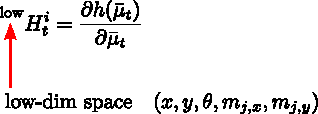
\includegraphics[width=0.4\textwidth]{ekf_slam/jacobian_observation.pdf}
        \end{center}
        %
        % \begin{equation*}
        %     \prescript{\text{low}}{}{H^{i}_{t}} = \frac{\partial h(\bar{\mu}_t)}{\partial \bar{\mu}_t}
        % \end{equation*}
        % \begin{equation*}
        %     \text{low-dim space} \quad (x, y, \theta, \map_{j,x}, \map_{j,y})
        % \end{equation*}

        We are only interested in the 5-dimension related with the observation.

    \end{itemize}
\end{frame}

\begin{frame}
    \frametitle{Jacobian for the Observation}
    \note{Información extraída de https://www.youtube.com/watch?v=X30sEgIws0g}
    \note{Información extraída de https://www.ipb.uni-bonn.de/html/teaching/photo12-2021/2021-pho2-16-ekf-slam.pptx.pdf}

    \begin{itemize}
        \item Based on
        \begin{align*}
            \delta &= 
            \begin{bmatrix}
                \delta_x \\
                \delta_y
            \end{bmatrix}
            = \begin{bmatrix}
                \bar{\mu}_{j,x} - \bar{\mu}_{t,x} \\
                \bar{\mu}_{j,y} - \bar{\mu}_{t,y}
            \end{bmatrix}\\
            q &= \delta^T \delta\\
            \hat{z}^i_t &= 
            \begin{bmatrix}
                \sqrt{q} \\
                \text{atan2}(\delta_y, \delta_x) - \bar{\mu}_{t,\theta}
            \end{bmatrix}
        \end{align*}    
        \item Compute the Jacobian
        \begin{align*}
            \prescript{\text{low}}{}{H^{i}_{t}} &= \frac{\partial h(\bar{\mu}_t)}{\partial \bar{\mu}_t}\\
            &= \begin{bmatrix}
                \frac{\partial \sqrt{q}}{\partial x} & \frac{\partial \sqrt{q}}{\partial y} & \cdots \\
                \frac{\partial \text{atan2}(\ldots)}{\partial x} & \frac{\partial \text{atan2}(\ldots)}{\partial y} & \cdots
            \end{bmatrix}
    \end{align*} 
    \end{itemize}

\end{frame}

\begin{frame}
    \frametitle{The first component}
    \note{Información extraída de https://www.youtube.com/watch?v=X30sEgIws0g}
    \note{Información extraída de https://www.ipb.uni-bonn.de/html/teaching/photo12-2021/2021-pho2-16-ekf-slam.pptx.pdf}

    \begin{itemize}
        \item Based on
        \begin{align*}
            \delta &= 
            \begin{bmatrix}
                \delta_x \\
                \delta_y
            \end{bmatrix}
            = \begin{bmatrix}
                \bar{\mu}_{j,x} - \bar{\mu}_{t,x} \\
                \bar{\mu}_{j,y} - \bar{\mu}_{t,y}
            \end{bmatrix}\\
            q &= \delta^T \delta\\
            \hat{z}^i_t &= 
            \begin{bmatrix}
                \sqrt{q} \\
                \text{atan2}(\delta_y, \delta_x) - \bar{\mu}_{t,\theta}
            \end{bmatrix}
        \end{align*}    
    
        \item We obtain (by applying the chain rule)
        \begin{align*}
            \frac{\partial \sqrt{q}}{\partial x}
            &= \frac{1}{2} \frac{1}{\sqrt{q}} 2 \delta_x (-1)\\
            &= \frac{1}{q} \left(-\sqrt{q} \delta_x \right)
        \end{align*} 
    \end{itemize}

\end{frame}

\begin{frame}
    \frametitle{Jacobian for the Observation}
    \note{Información extraída de https://www.youtube.com/watch?v=X30sEgIws0g}
    \note{Información extraída de https://www.ipb.uni-bonn.de/html/teaching/photo12-2021/2021-pho2-16-ekf-slam.pptx.pdf}

    \begin{itemize}
        \item Based on
        \begin{align*}
            \delta &= 
            \begin{bmatrix}
                \delta_x \\
                \delta_y
            \end{bmatrix}
            = \begin{bmatrix}
                \bar{\mu}_{j,x} - \bar{\mu}_{t,x} \\
                \bar{\mu}_{j,y} - \bar{\mu}_{t,y}
            \end{bmatrix}\\
            q &= \delta^T \delta\\
            \hat{z}^i_t &= 
            \begin{bmatrix}
                \sqrt{q} \\
                \text{atan2}(\delta_y, \delta_x) - \bar{\mu}_{t,\theta}
            \end{bmatrix}
        \end{align*}

        \item Compute the Jacobian
        
        \begin{align*}
            \prescript{\text{low}}{}{H^{i}_{t}} &= \frac{\partial h(\bar{\mu}_t)}{\partial \bar{\mu}_t}\\
            &= \frac{1}{q}
            \begin{bmatrix}
                -\sqrt{q} \delta_x & -\sqrt{q} \delta_y & 0 & \sqrt{q} \delta_x & \sqrt{q} \delta_y\\
                \delta_y & -\delta_x & -q & -\delta_y & \delta_x
            \end{bmatrix}
        \end{align*}
    \end{itemize}

\end{frame}

\begin{frame}
    \frametitle{Jacobian for the Observation}
    \note{Información extraída de https://www.youtube.com/watch?v=X30sEgIws0g}
    \note{Información extraída de https://www.ipb.uni-bonn.de/html/teaching/photo12-2021/2021-pho2-16-ekf-slam.pptx.pdf}

    \small

    \begin{itemize}
        \item Use the computed Jacobian
        \begin{align*}
            \prescript{\text{low}}{}{H^{i}_{t}} &= \frac{\partial h(\bar{\mu}_t)}{\partial \bar{\mu}_t}\\
            &= \frac{1}{q}
            \begin{bmatrix}
                -\sqrt{q} \delta_x & -\sqrt{q} \delta_y & 0 & \sqrt{q} \delta_x & \sqrt{q} \delta_y\\
                \delta_y & -\delta_x & -q & -\delta_y & \delta_x
            \end{bmatrix}
        \end{align*}
    
        \item Map it to the high dimensional space
        \begin{equation*}
            H^{i}_{t} = \prescript{\text{low}}{}{H^{i}_{t}} F_{x,j}
        \end{equation*}
        \begin{equation*}
            F_{x,j} =
            \begin{bNiceMatrix}[margin = 3 pt]
                1 & 0 & 0 & 0 \cdots 0 & 0 & 0 & 0 \cdots 0 \\
                0 & 1 & 0 & 0 \cdots 0 & 0 & 0 & 0 \cdots 0 \\
                0 & 0 & 1 & 0 \cdots 0 & 0 & 0 & 0 \cdots 0 \\
                0 & 0 & 0 & 0 \cdots 0 & 1 & 0 & 0 \cdots 0 \\
                0 & 0 & 0 & 0 \cdots 0 & 0 & 1 & 0 \cdots 0
                \CodeAfter
                \UnderBrace{5-4}{5-4}{2(j-1)}
                \UnderBrace{5-7}{5-7}{2(N-j)}
            \end{bNiceMatrix}
        \end{equation*} 
    \end{itemize}
\end{frame}

\begin{frame}
    \frametitle{Algoritmo de Filtro de Kalman Extendido}
    \note{Información extraída de https://www.youtube.com/watch?v=X30sEgIws0g}
    \note{Información extraída de https://www.ipb.uni-bonn.de/html/teaching/photo12-2021/2021-pho2-16-ekf-slam.pptx.pdf}
    
    \begin{algorithmic}[1]
    \Procedure{ExtendedKalmanFilter}{$\mu_{t-1}, \covariance_{t-1}, \controlCommand_{t}, \observation_{t}$}
        \State $\overline{\mu}_{t} = \motionModelFunction{\controlCommand_{t}, \mu_{t-1}}$
        \State $\overline{\covariance}_{t} = \motionModelJacobian_{t} \covariance_{t-1} \motionModelJacobian_{t}^{\top}+\motionParametersCovariance_{t}$
        \Statex
        \State $\alert{\kalmanGain_{t} = \overline{\covariance}_{t} \observationModelJacobian_{t}^{\top} (\observationModelJacobian_{t} \overline{\covariance}_{t}  \observationModelJacobian_{t} + \observationModelCovariance_{t})^{-1}}$
        \State $\alert{\mu_{t} = \overline{\mu}_{t} + \kalmanGain_{t} (\observation_{t} - \observationModelFunction{\overline{\mu}_{t}})}$
        \State $\alert{\covariance_{t} =  (I - \kalmanGain_{t} \observationModelJacobian_{t}) \overline{\covariance}_{t}}$
        \State \Return $\mu_{t}, \covariance_{t}$
    \EndProcedure
    \end{algorithmic}
\end{frame}

\begin{frame}
    \frametitle{EKF SLAM - Correction (1/2)}
    \note{Información extraída de https://www.youtube.com/watch?v=X30sEgIws0g}
    \note{Información extraída de https://www.ipb.uni-bonn.de/html/teaching/photo12-2021/2021-pho2-16-ekf-slam.pptx.pdf}

    \begin{algorithmic}[1]
        \Procedure{EKF\_SLAM\_Correction}{}
        \State $Q_t = \begin{bmatrix} \sigma_r^2 & 0 \\ 0 & \sigma_\theta^2 \end{bmatrix}$ \Comment{Measurement noise covariance}
        \For {all observed features $\observation_i^t = (r_i^t, \phi_i^t)^{\top}$}
            \State $j = c_i^t$ \Comment{data association somehow}
            \If{landmark $j$ never seen before}
                \State $\begin{bmatrix} \bar{\mu}_{j,x} \\ \bar{\mu}_{j,y} \end{bmatrix} = 
                       \begin{bmatrix} \bar{\mu}_{t,x} \\ \bar{\mu}_{t,y} \end{bmatrix} + 
                       \begin{bmatrix} r_i^t \cos(\phi_i^t + \bar{\mu}_{t,\theta}) \\ r_i^t \sin(\phi_i^t + \bar{\mu}_{t,\theta}) \end{bmatrix}$
                \Comment{Initialize new landmark position}
            \EndIf
            \State $\delta = \begin{bmatrix} \delta_x \\ \delta_y \end{bmatrix} = 
                   \begin{bmatrix} \bar{\mu}_{j,x} - \bar{\mu}_{t,x} \\ \bar{\mu}_{j,y} - \bar{\mu}_{t,y} \end{bmatrix}$
            \State $q = \delta^T \delta$
            \State $\hat{z}_i^t = \begin{bmatrix} \sqrt{q} \\ \operatorname{atan2}(\delta_y, \delta_x) - \bar{\mu}_{t,\theta} \end{bmatrix}$
                   \Comment{Predicted measurement}
        \algstore{ekf_slam_algorithm_break} % guarda el estado del argoritmo para que este pueda continuar en otro lugar
    \end{algorithmic}
\end{frame}

\begin{frame}
    \frametitle{EKF SLAM - Correction (2/2)}
    \note{Información extraída de https://www.youtube.com/watch?v=X30sEgIws0g}
    \note{Información extraída de https://www.ipb.uni-bonn.de/html/teaching/photo12-2021/2021-pho2-16-ekf-slam.pptx.pdf}

    \begin{algorithmic}[1]
        \algrestore{ekf_slam_algorithm_break} % continua el algoritmo de antes
        \State $F_{x,j} =
        \begin{bNiceMatrix}[margin = 3 pt]
            1 & 0 & 0 & 0 \cdots 0 & 0 & 0 & 0 \cdots 0 \\
            0 & 1 & 0 & 0 \cdots 0 & 0 & 0 & 0 \cdots 0 \\
            0 & 0 & 1 & 0 \cdots 0 & 0 & 0 & 0 \cdots 0 \\
            0 & 0 & 0 & 0 \cdots 0 & 1 & 0 & 0 \cdots 0 \\
            0 & 0 & 0 & 0 \cdots 0 & 0 & 1 & 0 \cdots 0
            \CodeAfter
            \UnderBrace{5-4}{5-4}{2j-2}
            \UnderBrace{5-7}{5-7}{2N-2j}
        \end{bNiceMatrix}$ \Comment{Jacobian of state mapping}
        \Statex
        \Statex
        \State $H_t^i = \frac{1}{q} \begin{bmatrix}
            -\sqrt{q} \delta_x & -\sqrt{q} \delta_y & 0 & \sqrt{q} \delta_x & \sqrt{q} \delta_y\\
            \delta_y & -\delta_x & -q & -\delta_y & \delta_x
        \end{bmatrix} F_{x,j}$ \Comment{Measurement Jacobian}
            
        \State $K_t^i = \bar{\Sigma}_t H_t^{i\top}(H_t^i \bar{\Sigma}_t H_t^{i\top} + Q_t)^{-1}$ \Comment{Kalman gain}
        \State $\bar{\mu}_t = \bar{\mu}_t + K_t^i(\observation_t^i - \hat{z}_t^i)$ \Comment{State update}
        \State $\bar{\Sigma}_t = (I - K_t^i H_t^i) \bar{\Sigma}_t$ \Comment{Covariance update}
        \EndFor
        \State $\mu_t = \bar{\mu}_t$ \Comment{Final state estimate}
        \State $\Sigma_t = \bar{\Sigma}_t$ \Comment{Final covariance estimate}
        \State \Return $\mu_t, \Sigma_t$ \Comment{Return updated state and covariance}
        \EndProcedure
    \end{algorithmic}
\end{frame}

\begin{frame}
    \frametitle{Implementation Notes}
    \note{Información extraída de https://www.youtube.com/watch?v=X30sEgIws0g}
    \note{Información extraída de https://www.ipb.uni-bonn.de/html/teaching/photo12-2021/2021-pho2-16-ekf-slam.pptx.pdf}

    \begin{itemize}
        \item Measurement update in a single step requires only one full belief update
        \item Always normalize angular components to be in $[-\pi,\pi]$. Otherwise this can screw up the jacobians.
        \item May not need to create $F$ matrices explicitly \note{you can manipulate the covarince matrix elements directly}
    \end{itemize}

    \note{As we describe the pseudo-code we need one full belief update for each observed landmark indepently. In Practivce, we can do a full belief update using all the landmarks that currently observed to speed up computation.}

\end{frame}

\begin{frame}
    \frametitle{Loop Closing}
    \note{Información extraída de https://www.youtube.com/watch?v=X30sEgIws0g}
    \note{Información extraída de https://www.ipb.uni-bonn.de/html/teaching/photo12-2021/2021-pho2-16-ekf-slam.pptx.pdf}

    \begin{itemize}
    \item Loop closing means revisiting (and recognizing) an already mapped area
    \item Data association under
    \begin{itemize}
        \item high ambiguity
        \item possible environment symmetries
    \end{itemize}
    \item Uncertainties collapse after a loop closure (whether the closure was correct or not)
    \item \alert{Wrong loop closures lead to filter divergence!}
    \end{itemize}
\end{frame}

\begin{frame}
    \frametitle{Before the Loop Closure}
    \note{Información extraída de https://www.youtube.com/watch?v=X30sEgIws0g}
    \note{Información extraída de https://www.ipb.uni-bonn.de/html/teaching/photo12-2021/2021-pho2-16-ekf-slam.pptx.pdf}

    \begin{center}
        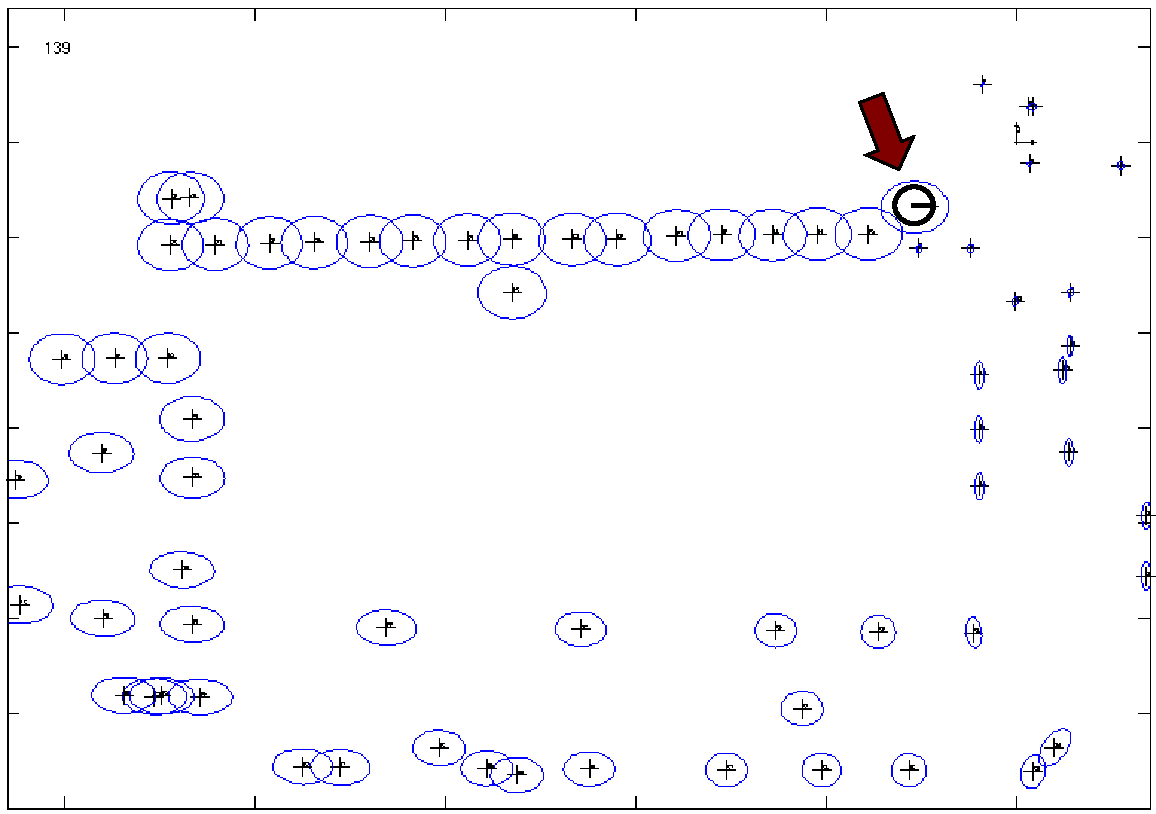
\includegraphics[width=0.6\textwidth]{ekf_slam/ekf_slam_loop_closure_before.pdf}
    \end{center}
\end{frame}

\begin{frame}
    \frametitle{After the Loop Closure}
    \note{Información extraída de https://www.youtube.com/watch?v=X30sEgIws0g}
    \note{Información extraída de https://www.ipb.uni-bonn.de/html/teaching/photo12-2021/2021-pho2-16-ekf-slam.pptx.pdf}

    \begin{center}
        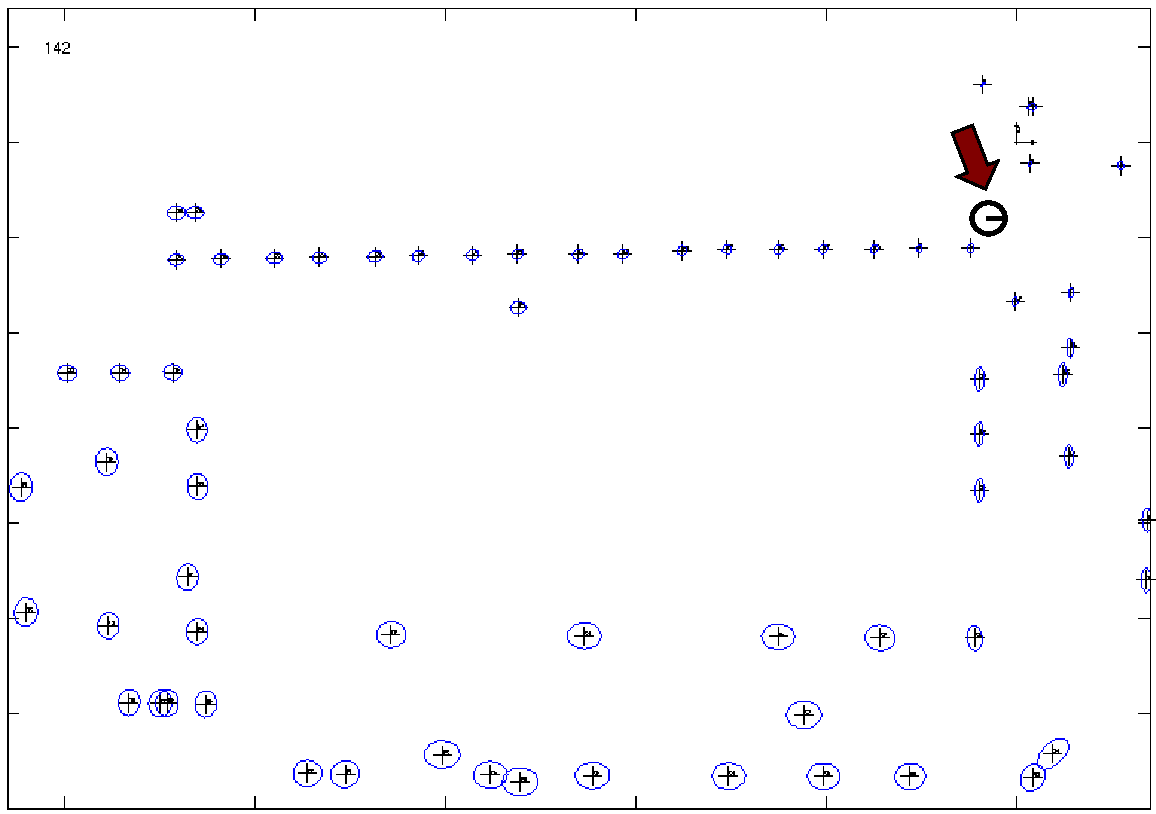
\includegraphics[width=0.6\textwidth]{ekf_slam/ekf_slam_loop_closure_after.pdf}
    \end{center}
\end{frame}

\begin{frame}
    \frametitle{Loop Closing}
    \note{Información extraída de https://www.youtube.com/watch?v=X30sEgIws0g}
    \note{Información extraída de https://www.ipb.uni-bonn.de/html/teaching/photo12-2021/2021-pho2-16-ekf-slam.pptx.pdf}

    \begin{itemize}
    \item Loop closing reduces the uncertainty in robot and landmark estimates
    \item This can be exploited when exploring an environment for the sake of better (e.g. more accurate) maps
    \item Wrong loop closures lead to filter divergence
    \end{itemize}
\end{frame}

\begin{frame}
    \frametitle{EKF SLAM Correlations}
    \note{Información extraída de https://www.youtube.com/watch?v=X30sEgIws0g}
    \note{Información extraída de https://www.ipb.uni-bonn.de/html/teaching/photo12-2021/2021-pho2-16-ekf-slam.pptx.pdf}

    \begin{itemize}
        \item In the limit, the landmark estimates become fully correlated
    \end{itemize}

    \begin{center}
        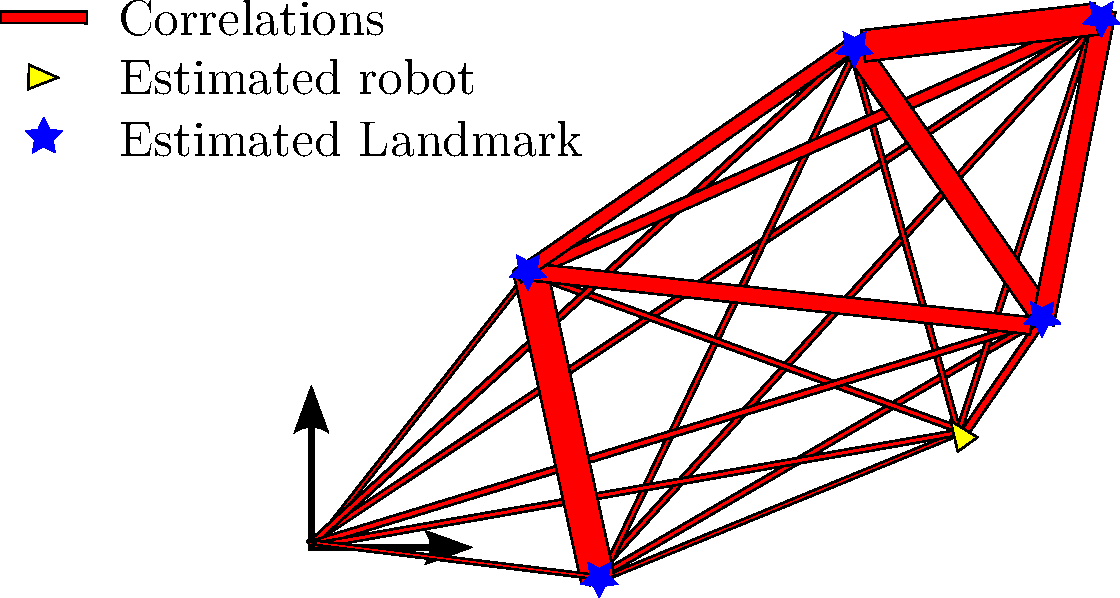
\includegraphics[width=0.45\textwidth]{../images/ekf_slam/ekf_slam_correlations.pdf}
    \end{center}

    \scriptsize

    \begin{itemize}
        \item In the long run all the estimates are fully correlated. All the landmark locations are fully (and strongly) correlated with each other (thick lines) and the pose is correlated with the landmarks in a weaker manner (thin lines).
        \item The Covariance Matrix represents the uncertainty and correlation between different state variables (e.g., robot pose and positions of landmarks). The \textbf{correlation matrix} is the normalized covariance matrix of the posterior estimate.
        \begin{itemize}
            \item Diagonal: Variance (uncertainty) of each variable.
            \item Off-diagonal: Correlation between variables (how errors in one affect another).
        \end{itemize}
    \end{itemize}

    \note{The correlation matrix simply divides the covariance of the two variables by the product of their standard deviations.}
    
\end{frame}

\begin{frame}
    \frametitle{EKF SLAM Correlations}
    \note{Información extraída de https://www.youtube.com/watch?v=X30sEgIws0g}
    \note{Información extraída de https://www.ipb.uni-bonn.de/html/teaching/photo12-2021/2021-pho2-16-ekf-slam.pptx.pdf}

    \begin{center}
        \only<1>{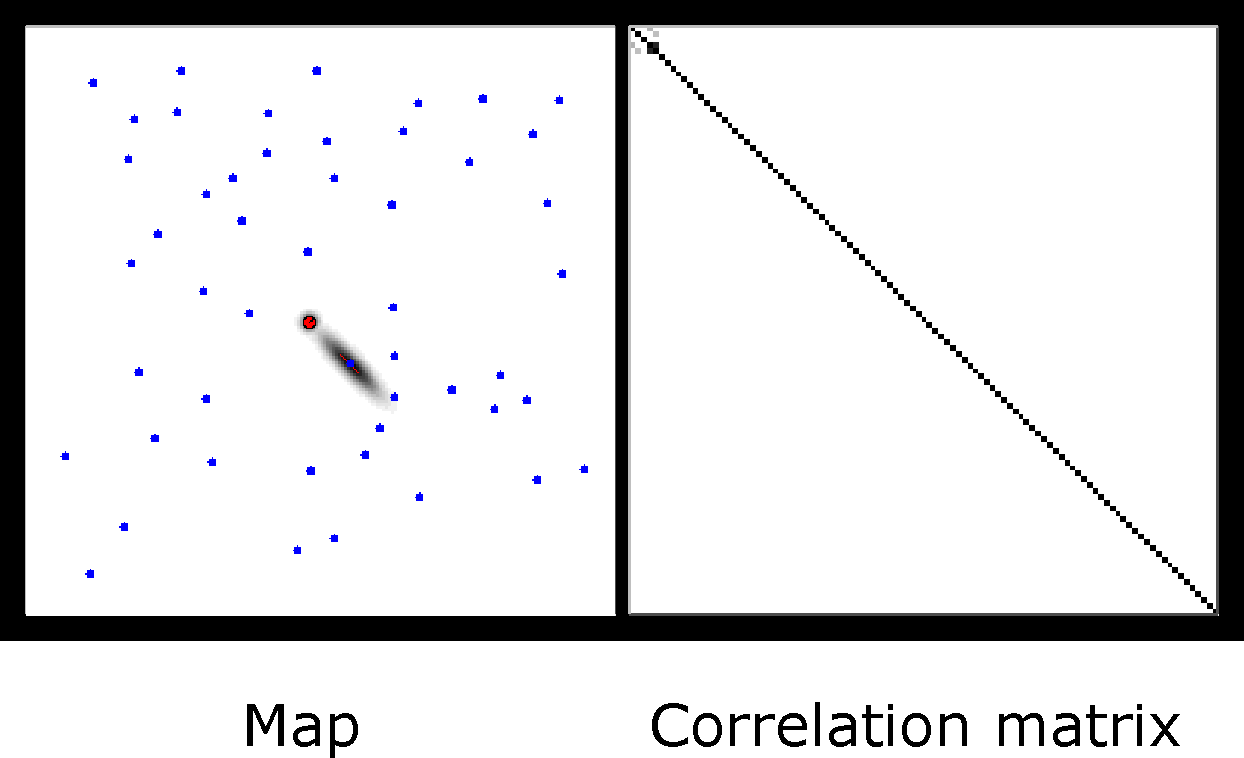
\includegraphics[width=0.8\textwidth]{../images/ekf_slam/ekf_slam_correlation_matrix1.pdf}}
        \only<2>{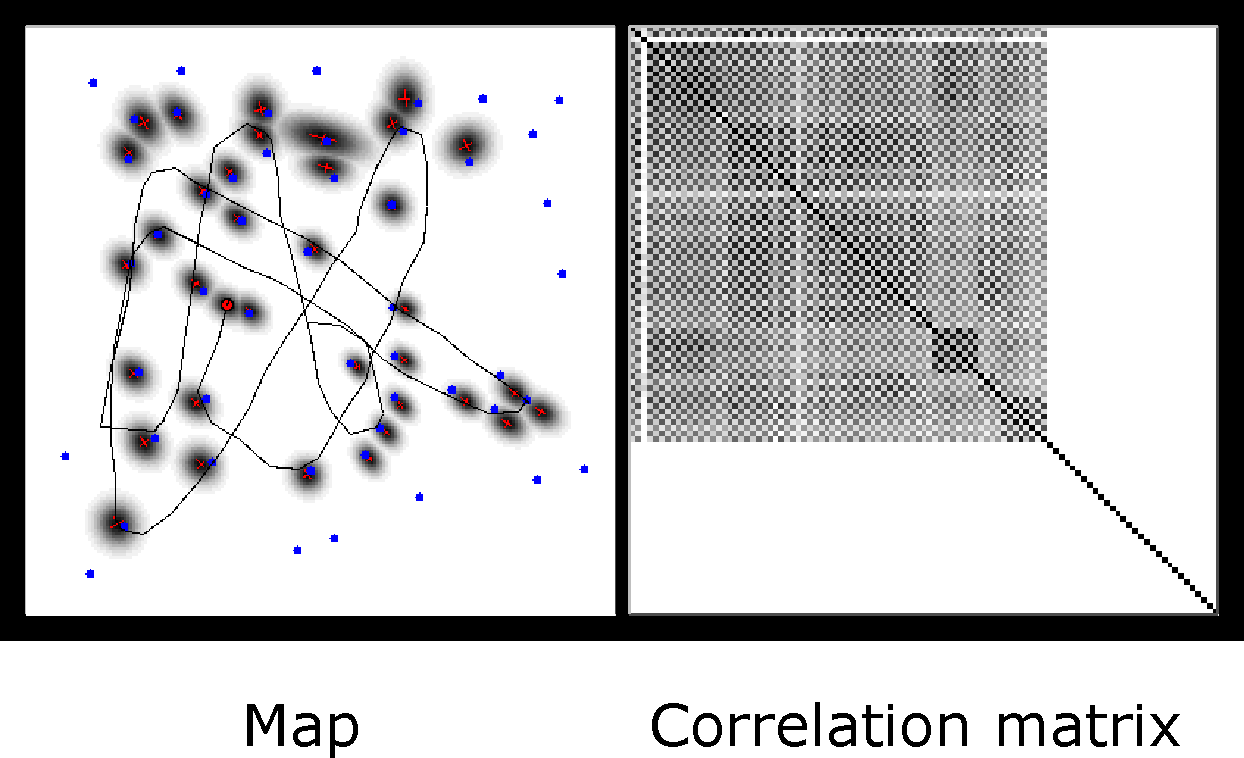
\includegraphics[width=0.8\textwidth]{../images/ekf_slam/ekf_slam_correlation_matrix2.pdf}}
        \only<3>{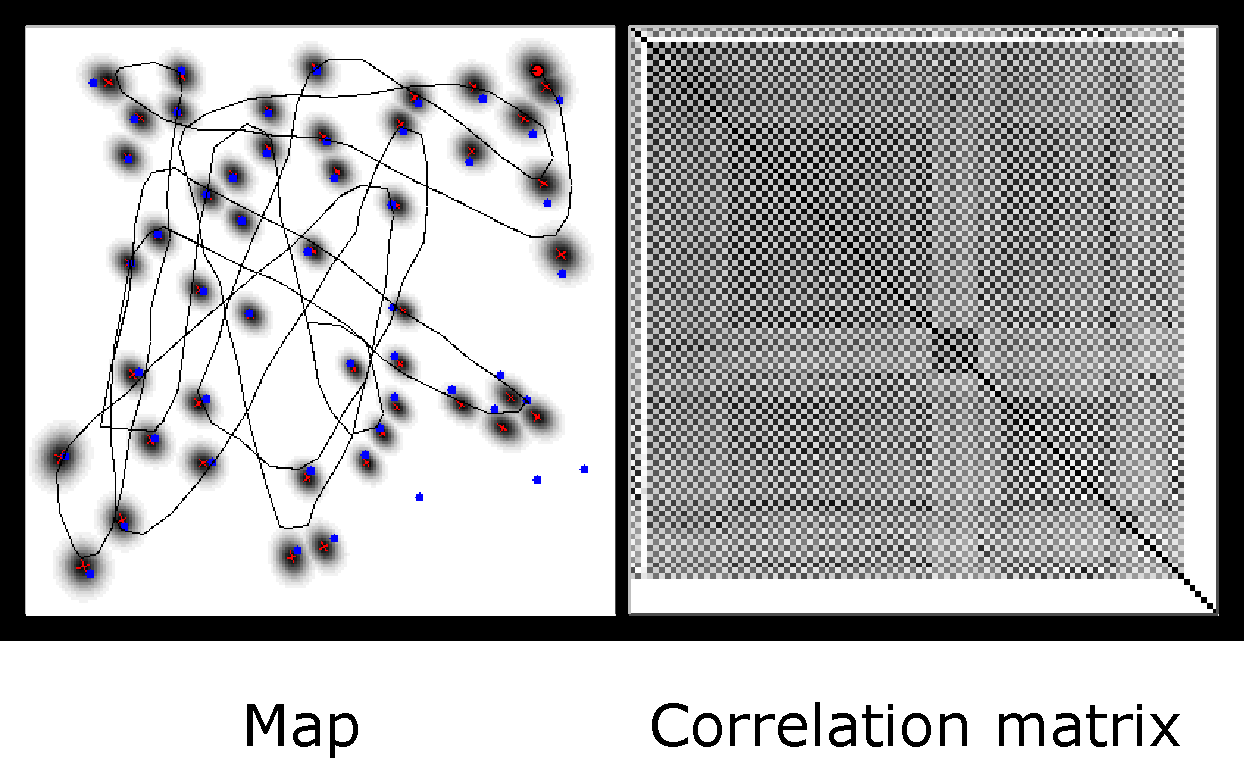
\includegraphics[width=0.8\textwidth]{../images/ekf_slam/ekf_slam_correlation_matrix3.pdf}}
    \end{center}

    \note{The while line (zero values) in the third row and column of the correlation matrix comes from the orientation. This means the robot orientation is not correlated with the lanmarks positions.}

    \note{Note that the correlation matrix looks like a checkboard. This is because, in the map, each landmark has a covariance that is mosly a circle, so the 2x2 landmarks covariance block of the main diagonal of the correlation matrix, off-diagonal elements of such 2x2 block are close to zero.
    On the other hand, for the off-diagonal elements of the correlation matrix, if I would be able to fix the x component location of one landmark, so I could dramatically reduce the uncertainty about the x location of all the other landmarks as well, because through the estimate Iquite of rigitdly connected those landmarks so if I shift one landmark with high uncertainty with zero uncertainty then all the map will shift as well. Therefore, if know the precise x location of a landmark I will know all the x locations of all other landmarks as well but I not learn anything about y.}

\end{frame}

\begin{frame}
    \frametitle{EKF SLAM Correlations}
    \note{Información extraída de https://www.youtube.com/watch?v=X30sEgIws0g}
    \note{Información extraída de https://www.ipb.uni-bonn.de/html/teaching/photo12-2021/2021-pho2-16-ekf-slam.pptx.pdf}

    \begin{itemize}
        \item The correlation between the robot's pose and the landmarks \textbf{cannot} be ignored 
        \item Assuming independence generates too optimistic estimates of the uncertainty
    \end{itemize}

    \note{So if you ignore the correlations you will be too optimistic since this means that you are setting all the other uncertainty values to zero.}

\end{frame}

\begin{frame}
    \frametitle{EKF SLAM Uncertainties}
    \note{Información extraída de https://www.youtube.com/watch?v=X30sEgIws0g}
    \note{Información extraída de https://www.ipb.uni-bonn.de/html/teaching/photo12-2021/2021-pho2-16-ekf-slam.pptx.pdf}

    \begin{itemize}
    \item The \textbf{determinant} of any sub-matrix of the map covariance matrix \textbf{decreases monotonically}
    \item New landmarks are initialized with \textbf{maximum uncertainty}
    \end{itemize}

    \begin{center}
        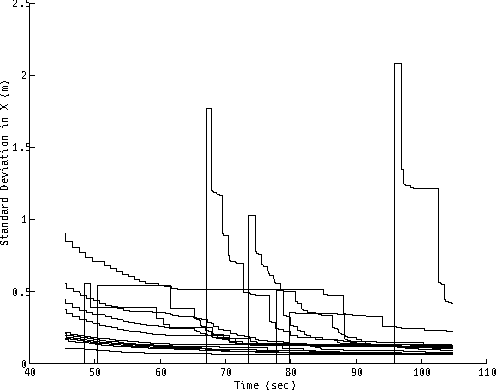
\includegraphics[width=0.5\textwidth]{../images/ekf_slam/landmarks_uncertainty_decrease.pdf} % Replace with actual vectorized image
    \end{center}
\end{frame}

\begin{frame}
    \frametitle{EKF SLAM in the Limit}
    \note{Información extraída de https://www.youtube.com/watch?v=X30sEgIws0g}
    \note{Información extraída de https://www.ipb.uni-bonn.de/html/teaching/photo12-2021/2021-pho2-16-ekf-slam.pptx.pdf}
    
    \begin{itemize}
        \item In the limit, the covariance associated with any single landmark location estimate is determined only by the initial covariance in the vehicle location estimate.
    \end{itemize}

    \begin{center}
        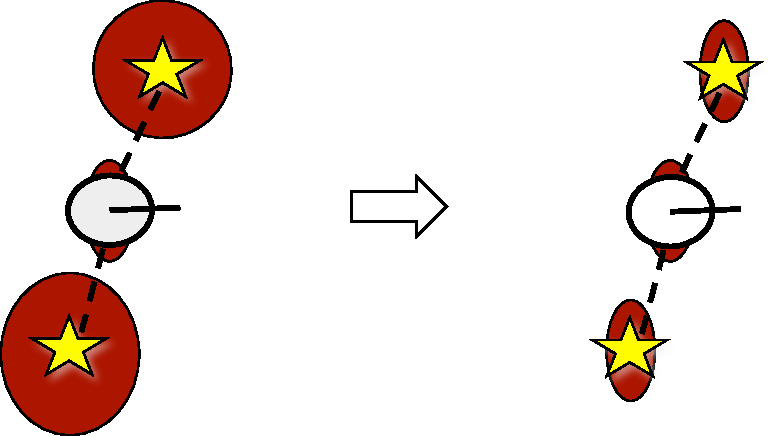
\includegraphics[width=0.6\textwidth]{../images/ekf_slam/ekf_slam_limit.pdf}
    \end{center}

\end{frame}

\begin{frame}
    \frametitle{EKF-SLAM 2D Example}
    \note{Vídeo extraído de https://youtu.be/xXo5oBYnuxE?si=VGVFflbAgcABIIVf}
    \note{https://github.com/taihup/slam_ekf_ros2}
        
    \begin{center}
    \movie[poster,loop,showcontrols]{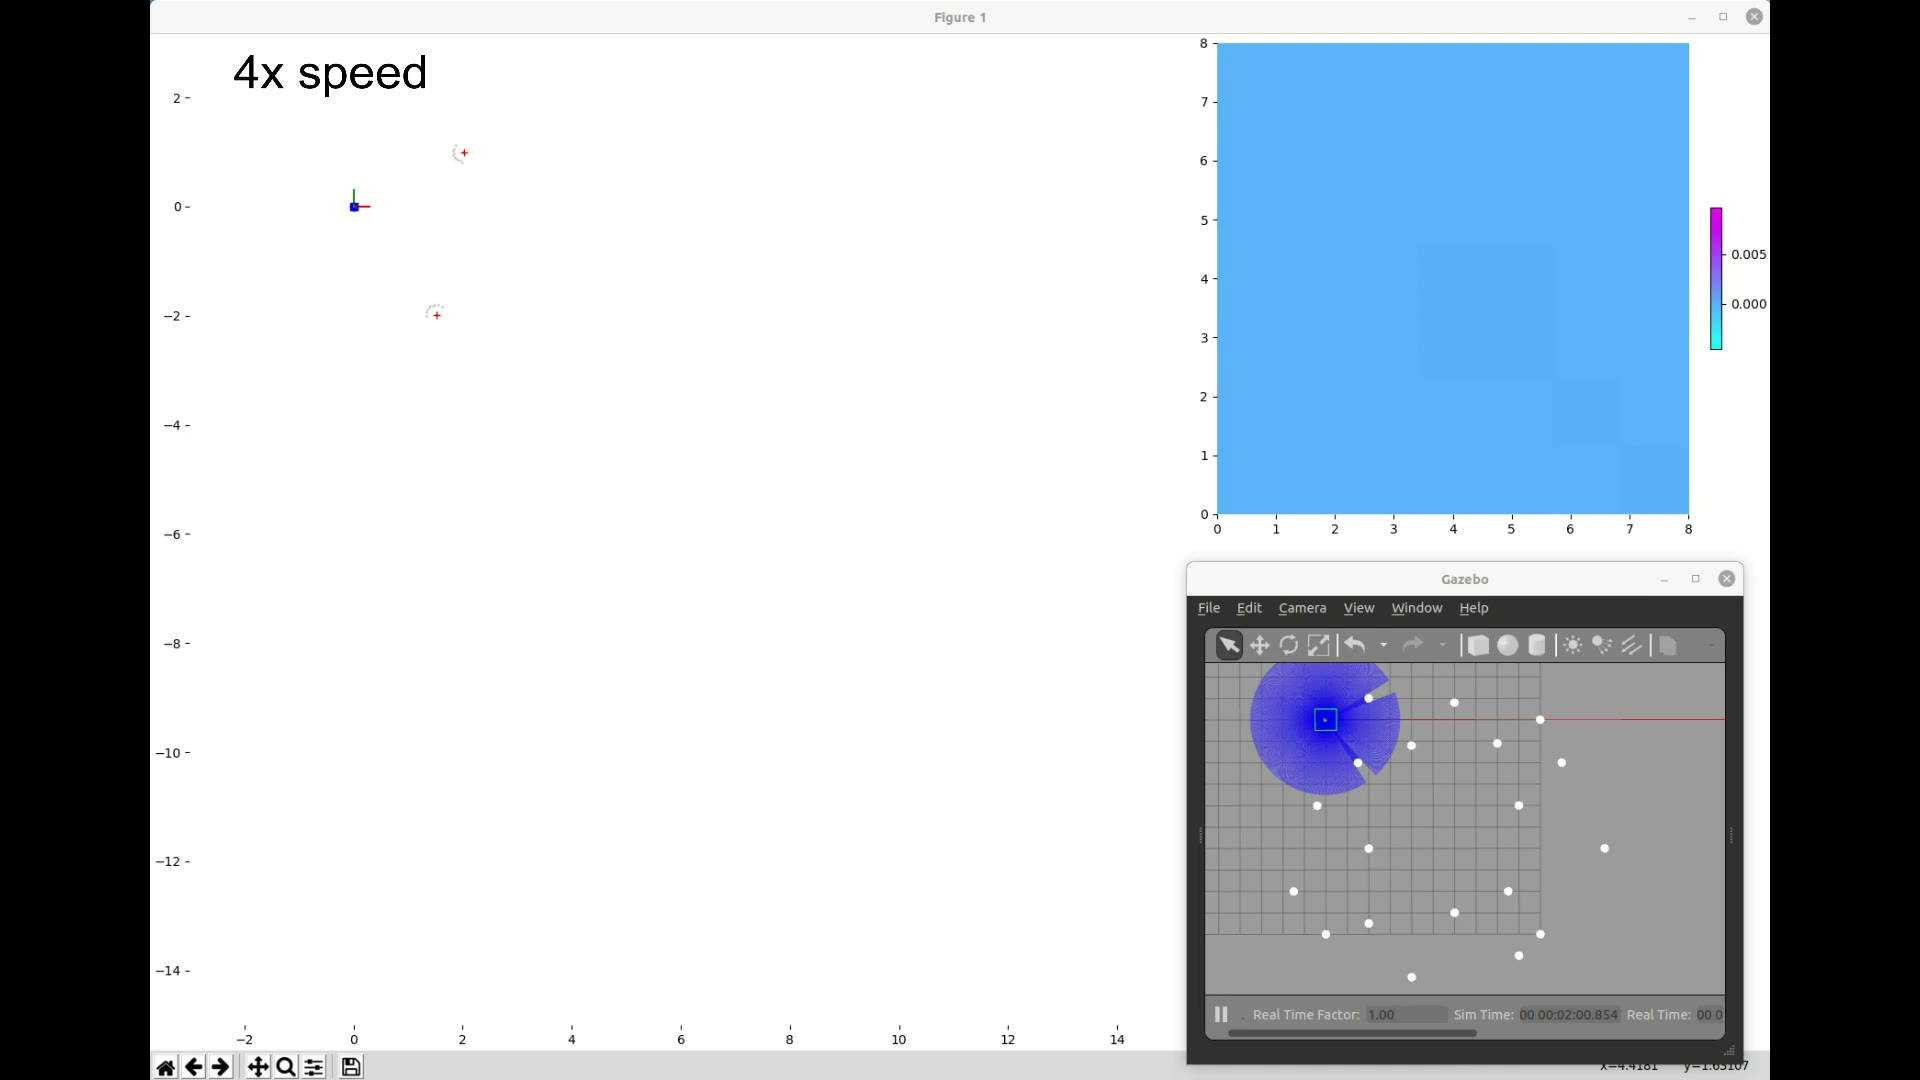
\includegraphics[width=0.9\columnwidth]{./images/ekf_slam/ekf_slam_2d_video.jpg}}{./videos/ekf_slam_2d.mp4}
    \end{center}

    \note{The covariance matrix is shown in the upper-left corner.}

\end{frame}

\begin{frame}
    \frametitle{EKF SLAM Complexity}
    \note{Información extraída de https://www.youtube.com/watch?v=X30sEgIws0g}
    \note{Información extraída de https://www.ipb.uni-bonn.de/html/teaching/photo12-2021/2021-pho2-16-ekf-slam.pptx.pdf}

    \begin{itemize}
    \item Cubic complexity w.r.t. measurement dimensionality \note{and not w.r.t the whole state, this is because you are only observing small number of landmark and not the whole map.}
    \item Cost per step: $O(n^2)$ (dominated by number of landmarks)
    \item Memory consumption: $O(n^2)$
    \item Computationally intractable for large maps!
    \end{itemize}
\end{frame}

\begin{frame}
    \frametitle{EKF SLAM Summary}
    \note{Información extraída de https://www.youtube.com/watch?v=X30sEgIws0g}
    \note{Información extraída de https://www.ipb.uni-bonn.de/html/teaching/photo12-2021/2021-pho2-16-ekf-slam.pptx.pdf}

    \begin{itemize}
    \item First probabilistic SLAM approach using EKF
    \item Convergence proof for the linear Gaussian case
    \item Can diverge if non-linearities are large
    \item The smaller the noise the better
    \item Unimodal (Gaussian) estimates only \note{EKF can not handle multimodal uncertainty. Eg: I cannot say either the landmark is here or there but I don't exatly know. Particle filter can!}
    \item Successful in medium-scale scenes
    \item Used for short-term estimates (VO)
    \item Approximations exists to reduce the computational complexity
    
    \end{itemize}
\end{frame}

\begin{frame}
    \frametitle{Literature}
    \note{Información extraída de https://www.youtube.com/watch?v=X30sEgIws0g}
    \note{Información extraída de https://www.ipb.uni-bonn.de/html/teaching/photo12-2021/2021-pho2-16-ekf-slam.pptx.pdf}

    \begin{itemize}
    \item Thrun et al.: "Probabilistic Robotics", Chapter 10
    \end{itemize}
\end{frame}